\documentclass{article}
% Language setting
% Replace `english' with e.g. `spanish' to change the document language
\usepackage[english]{babel}
% Set page size and margins
% Replace `letterpaper' with `a4paper' for UK/EU standard size
\usepackage[letterpaper,top=2cm,bottom=2cm,left=3cm,right=3cm,marginparwidth=1.75cm]{geometry}
% Useful packages
\usepackage{multicol}
\usepackage{amsmath}
\usepackage{amssymb}
\usepackage{graphicx}
\usepackage[framemethod=tikz]{mdframed}
\usepackage{array}
\usepackage{blindtext}
%\usepackage[paperwidth=10cm]{geometry}
\usepackage{tkz-euclide}
%\usepackage{tikz}
\usetikzlibrary{
  circuits.logic,
  circuits.logic.US,
  positioning
}

\usepackage[colorlinks=true, allcolors=blue]{hyperref}
\newcommand{\myvec}[1]{\ensuremath{\begin{pmatrix}#1\end{pmatrix}}}
\providecommand{\norm}[1]{\left\lVert#1\right\rVert}
\let\vec\mathbf
\title{Optimization Assignment-1}
\author{T. Varsha Reddy}
\begin{document}
\maketitle
\newtheorem{theorem}{Theorem}[section]
\begin{multicols}{2}

\paragraph{\begin{flushleft}\textbf{Problem: }
\textbf{One kind of cake requires 300gm of flour and 15gm of fat and another kind of cake requires 150gm  of flour and 30gm  of fat. Find the maximum number of cake that can be made from 7.5kg  of flour and 600gm  of fat . Form a linear programming problem and solve it graphically.}
\end{flushleft}}
\resizebox{6.5cm}{!}
{
\begin{tabular}{|c|c|c|}
	\hline
	\textbf{Food}&\textbf{Cake A}&\textbf{Cake B}\\
	\hline
	\textbf{X}&300&150\\
	\hline
	\textbf{Y}&15&30\\
	\hline
\end{tabular}}
\begin{flushleft}
\textbf{Given that first kind of cake requires 15g of fat while second kind of cake required 30g of fat.}
\end{flushleft}
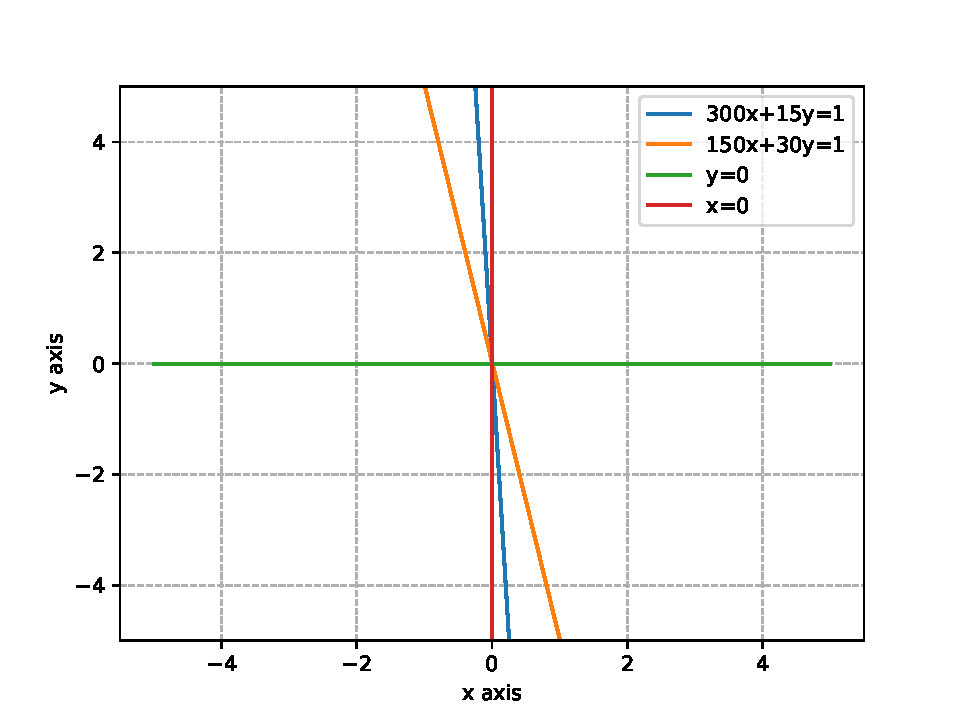
\includegraphics[scale=0.5]{opt1.pdf} 
\section*{Solution}
\begin{flushleft}
Let mixture contains x units of food X,y units of food Y.\\
According to given problem, problem can be formulated as,\\
\end{flushleft}
\begin{align}
P=max(7500x+600y)
\end{align}
where P is maximum cost of Cake A
\begin{align}
300x+15y \geq1
\end{align}
for Cake B
\begin{align}
150x+30y \geq 1
\end{align}
%for Vitamin C
%\begin{align}
%3x+y \geq 8
%\end{align}
mixture contains both X,Y so,
\begin{align}
x\geq0,y\geq0
\end{align}
eq 1 and 2 to 4 can be expressed in vector form as
\begin{align*}
\vec{P}=max\myvec{7500 \hspace{0.2cm}600}\vec{x}\\
\myvec{300 \hspace{0.2cm} 15\\
       150 \hspace{0.2cm} 30\\
      % 3 \hspace{0.2cm} 1\\
       1 \hspace{0.2cm}0\\
       0 \hspace{0.2cm} 1}\vec{x}\geq \myvec{1 \\1\\0\\0}
\end{align*}
Solving above equations using cvxpy, we get\\
\begin{center}
$P_{max}$=30\\
\end{center}
\begin{center}
$\vec{x}$=$\myvec{0.0022\\0.0222}$
\end{center}
\end{multicols}{2}
\end{document}